\section{Grundlagen und Ansätze der Virtualisierung von Testumgebungen}

Laut Duden leitet sich das Adjektiv "`virtuell"' vom lateinischen "`virtus"' für "`Kraft, Tugend, Männlichkeit"' ab. Es bedeutet so viel wie "`von unwirklicher, scheinbarer, nicht tatsächlicher Form"'.

Innerhalb der Informatik kann man von zwei unterschiedlichen Arten der Virtuatlität sprechen. Zum einen gibt es den Bereich der "virtuellen Realität", bei der einem Menschen mit Hilfe einer in Echtzeit computergenerierten Umgebung das Gefühl vermittelt wird, sich in einer anderen Wirklichkeit zu befinden. Zum anderen gibt es eben den Bereich der Virtualisierung, bei dem es darum geht, einem Anwender (Mensch oder auch Programm) bestimmte Rahmenbedingungen vorzuspielen, die so eigentlich nicht existieren.

Ein einfaches Beispiel für Virtualisierung sind Hardware-Emulatoren. Hardware-Emulatoren gaukeln Software vor, mit einer Hardware zu interagieren, die so physisch gar nicht existiert. Dies wird z.B. verwendet, um alte Spiele von nicht mehr produzierten Spielekonsolen auf aktuellen Computern auszuführen oder auch um Apps für mobile Geräte wie Smartphones oder Tablets auf Desktoprechnern zu entwickeln oder zu testen, ohne diese Geräte wirklich vorzuhalten.

Ein weiteres Beispiel ist die Virtualisierung von Netzwerkressourcen. So können z.B. VLANs (Virtual Local Area Networks) verbundenen Geräten eine ganz andere Verkabelung vorgaukeln als sie physikalisch vorliegt, um so bestimmte Zugriffe zu erlauben oder zu sperren.

Der für diese Arbeit interessante Bereich der Virtualisierung ist das Bereitstellen virtueller Betriebsumgebungen. Eine Betriebsumgebung meint die Umgebung, die ein Programm für seine Ausführung benötigt. Dazu gehören vor allem bestimmte Hardware-Bauteile (Prozessoren, Arbeitsspeicher, Festplatten, Netzwerk-Adapter), ein Betriebssystem und eventuell zusätzliche Anwendungsprogramme, mit denen das Programm interagiert. Für gewöhnlich läuft eine solche Betriebsumgebung genau auf einem Rechner (z.B. Server oder Desktoprechner). Es gibt nun verschiedene Ansätze eine solche Betriebsumgebung zu virtualisieren, die sich hinsichtlich ihrer Implementierung und Funktionalität unterscheiden. Grundsätzlich unterscheidet man zwischen der Systemvirtualisierung mittels Hypervisor und der Betriebssystemvirtualisierung mittels OS-Containern. Auf diese Varianten soll nun im Näheren eingegangen werden, um so mögliche Kandidaten für die Virtualisierung von Testumgebungen gemäß der Problemstellung zu finden. Abschließend wird ein kurzer Vergleich der beiden Varianten durchgeführt.

\begin{figure}[!ht]
  \begin{center}
    \includegraphics[width=8cm]{bilder/Einordnung_Virtualisierungstechnologien_für_virtuelle_Betriebsumgebungen.png}
    \caption{Einordnung Virtualisierungtechnologienen für virtuelle Betriebsumgebungen \citep{Hirschbach06}}
  \end{center}
\end{figure}

\subsection{Systemvirtualisierung mittels Hypervisor}

Als Hypervisor oder auch \ac{VMM} wird eine Software bezeichnet, die die physisch vorhandene Hardware abstrahiert und mehreren Gastbetriebssystemen zur Verfügung stellt. Dabei spielt es den Gastsystemen jeweils vor, dass sie auf einem eigenen vollständigen Rechner mit Prozessor, Arbeitsspeicher, Festplatte und sonstigen Geräten laufen. Ein solcher virtueller Rechner wird auch \ac{VM} genannt. Je nach tatsächlich vorhandener Hardware muss der \ac{VMM} dabei die Hardware für das Gastsystem emulieren, virtualisieren oder paravirtualisieren. Emulieren meint hierbei, das der \ac{VMM} dem Gastsystem eine Hardware anbietet, die garnicht existiert. Virtualisieren meint, dass er Zugriffe des Gastsystems auf die virtuelle Hardware entsprechend auf die physische Hardware übersetzt. Paravirtualisierung findet dann statt, wenn die physische Hardware selbst das Konzept der Virtualisierung versteht und die Zugriffe des Gastsystems zumindest teilweise selbst verarbeiten kann. Hierbei unterscheiden sich die unterschiedlichen Ansätze natürlich vorallem hinsichtlich ihrer Performance, da das Übersetzen der Zugriffe oder das komplette Emulieren einer Hardware aufwendiger ist, als direkt auf die Hardware zuzugreifen.

Man kann diesen Unterschied in der Zugriffsart zum Beispiel anhand der Ring-Schemas aktueller Prozessoren verdeutlichen. Ein Ring bezeichnet dabei eine Sicherheitsstufe eines Prozesses, der vom Prozessor verarbeitet wird. Je nach Sicherheitsstufe darf der Prozess dabei auf mehr oder weniger Befehlssätze innerhalb des Prozessors zugreifen. Solche Befehlssätze beinhalten zum Beispiel Befehle zum Kopieren von Daten (Transferbefehle) innerhalb des Systems oder auch arithmetische Befehle zur Verrechnung von Werten. Der Ring 0 bezeichnet dabei nun die Sicherheitsstufe, innerhalb derer ein Prozess auf alle Befehlssätze des Prozessors zugreifen darf. Man nennt diesen Ring auch "`Kernel-Mode"', da in diesem Modus typischerweise nur das Betriebssystem bzw. dessen Kern, der sogenannter Kernel, ausgeführt wird. Prozesse normaler Anwendungsprogramme werden hingegen in Ring 3 ausgeführt, der nur wenige Befehlssätze ausführen darf. Man nennt diesen Ring auch "`User-Mode"'. Ein Prozess im Ring 3 darf zum Beispiel keine Transferbefehle ausführen. Benötigt er entsprechende Operationen, greift er auf Funktionen des Kernels des Betriebssystems zu, die dabei bestimmte Berechtigungen sicherstellen können. Ein Prozess in Ring 3 kann somit zum Beispiel nicht auf den Arbeitsspeicher anderer Prozesse zugreifen oder sich selbst in einen anderen Ausführungsmodus bringen \citep[Vgl.][]{wiki:005}.

\begin{figure}[!ht]
  \begin{center}
    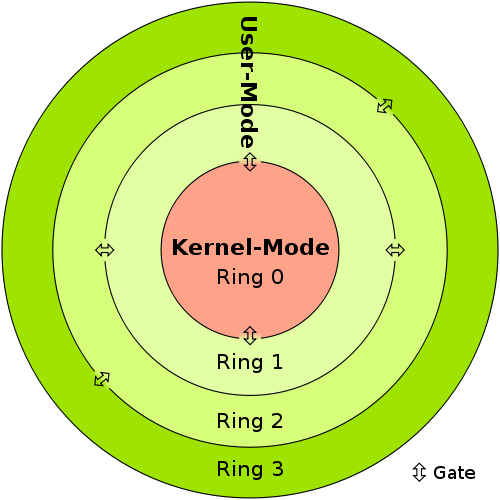
\includegraphics[width=6cm]{bilder/500px-CPU_ring_scheme.png}
    \caption{CPU Ring scheme \citep{wiki:006}}
  \end{center}
\end{figure}

Wenn man nun ein Betriebssytem in einer virtuellen Maschine ausführen möchte, versucht dieses wiederrum Befehle aus dem Befehlssatz des Ring 0 zu rufen, obwohl die Gastmaschine als Prozess in Ring 3 ausgeführt wird. Hypervisoren lösen dieses Problem nun grundsätzlich so, dass sie den Code, der innerhalb der virtuellen Maschine und somit in Ring 3 läuft, nach Befehlen durchsuchen, die nicht ausführbar sind. Diese Befehle werden dann im Speicher durch erlaubte Aufrufe ersetzt. Eine Möglichkeit ist es hierbei, den nicht erlaubten Befehl durch einen entsprechenden Aufruf an den Hypervisor zu ersetzen, der daraufhin einen entsprechenden Aufruf an das Betriebssystem vornimmt. Dies ist eben die ineffizienteste Variante. Moderne Prozessoren bieten nun aber spezielle Befehle zur Virtualisierung an, die nicht nur aus dem Ring 0 gerufen werden können. Hypervisoren nutzen diese aus, indem Sie den Code des Gastbetriebssystem scannen und die entsprechenden Aufrufe auf Ring 0 im Speicher durch solche ersetzen, die auf die spezialisierten Virtualisierungsbefehlsätze zeigen. Dies wäre dann keine emulierter Prozessor sondern eben ein virtualisierter Prozessor, da die zugrunde liegende Hardware direkt wiederverwendet wird. Moderne Betriebssysteme und Hypervisoren kommen damit auf Ausführungszeiten, die nahezu denen auf direkter physischer Hardware entsprechen.

Robert P. Goldberg, der die Grundlagen des \ac{VMM} in den 70er Jahren wissenschaftlich erarbeitet hat, unterscheidet in seiner Doktorarbeit "`Architectural Principles for Virtual Computer Systems"' nun zwei Klassen des \ac{VMM} \citep[vgl.][S. 22 ff.]{Goldberg73}: Dem Typ I \ac{VMM} oder auch "`Bare Metal Hypervisor"' und dem Typ II \ac{VMM} oder auch "`Hosted Hypervisor"'. In den folgenden beiden Unterkapiteln sollen diese beiden Klassen und entsprechende Implementierungen näher beleuchtet werden.

Darauf folgt abschließend ein Unterkapitel zu den sogenannten Unikernels, einer relativ neuen Entwicklung innerhalb der Systemvirtualisierung mittels Hypervisor, die eine bestimmte Art von \ac{VM} beschreibt \citep[siehe Abstract]{MadMorAnd13}.

\subsubsection{Bare Metal Hypervisors}

Ein Bare Metal Hypervisor ist ein \ac{VMM}, der als eigenständiges Programm direkt auf echter physischer Hardware läuft und somit kein Betriebssystem auf dem Hostsystem benötigt.

\begin{figure}[!ht]
  \begin{center}
    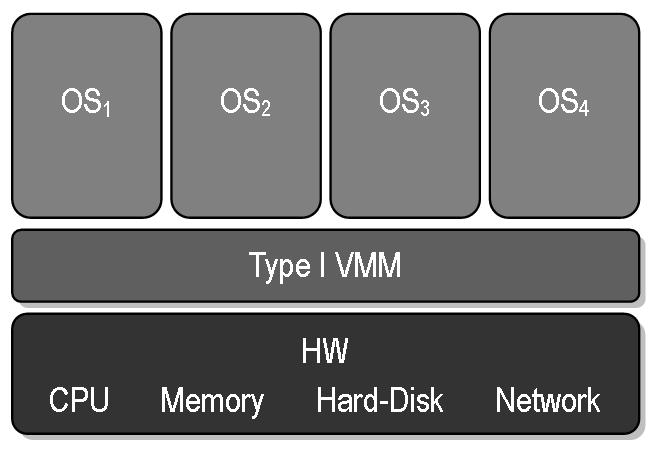
\includegraphics[width=6cm]{bilder/VMM-Type1.jpg}
    \caption{Virtual Machine Monitor Type I \citep{wiki:002}}
  \end{center}
\end{figure}

Durch diesen direkten Zugriff und das nicht notwendige Hostbetriebssystem gilt ein Bare Metal Hypervisor als ressourceneffizienter als ein Hosted Hypervisor. Größter Nachteil dieser Variante ist aber, dass sie mit mehr Installationsaufwand verbunden ist, da der Hypervisor selbst die passenden Gerätetreiber für die zugrundeliegende Hardware benötigt und man nicht auf Standardwerkzeuge wie zum Beispiel den Installationsmanagers eines Hostbetriebssystems zugreifen kann. Typische Vertreter dieser Hypervisor-Klasse sind zum Beispiel KVM und Citrix XenServer  \citep{wiki:004}.

Beim Open-Source-Produkt KVM (Kernel-based Virtual Machine) handelt es sich um eine Lösung, bei der ein normaler Linux-Kernel über ein spezielles Kernel-Modul für die grundsätzliche Virtualisierung (kvm.io) und ein weiteres prozessorspezifisches Kernel-Modul (kvm-intel.io oder kvm-amd.io) in die Lage versetzt wird, als Hypervisor zu arbeiten und Gastsysteme zu verwalten. KVM lässt sich damit grundsätzlich auf allen gängigen Linux Distributionen installieren. Oft wird deshalb vermutet, dass es sich nicht um einen reinen Bare Metal Hypervisor handelt, da er eben zusammen mit einem Betriebssystem installiert wird. Da es sich bei dem Kernel-Modul aber nicht um ein Anwendungsprogramm handelt, sondern um eine Erweiterung des eigentlichen Kernels, setzt diese Virtualisierungslösung direkt auf der darunterliegenden Hardware und nicht auf einem dazwischenliegenden Kernel auf \citep[Vgl.][]{kvm:001}.

\begin{figure}[!ht]
  \begin{center}
    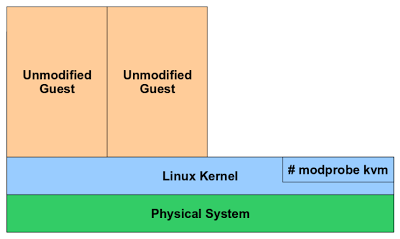
\includegraphics[width=8cm]{bilder/kvm.png}
    \caption{KVM Architektur \citep{kvm:002}}
  \end{center}
\end{figure}

So gibt es zum Beispiel die Linux Distribution Proxmox VE, die man direkt auf eine leere Hardware installieren kann und die die entsprechenden Kernel-Module und weitere Hilfsprogramme (zum Beispiel zur Verwaltung der virtuellen Maschinen) bereits beinhaltet \citep[Vgl.][]{Proxmox14}.

Auch bei XenServer von der Firma Citrix handelt es sich um ein Open-Source-Produkt. Auch dieser \ac{VMM} setzt direkt auf der eigentlichen physischen Hardware auf. XenServer basiert ebenfalls auf einem Linux-Kernel. Es handelt sich aber nicht lediglich um Kernel-Module, die sich in eine beliebige Linux-Distribution laden lassen sondern um einen modifizerten Linux-Kernel. XenServer lässt sich also nur auf komplett leere Hardware installieren und bietet auch nicht die vollständigen Funktionalitäten einer normalen Linux-Distribution. Das besondere an XenServer ist, dass die Prozesse zur Steuerung der virtuellen Maschinen selbst in einer virtuellen Maschine laufen. Diese auch "`Privileged Guest"' genannte Maschine muss laufen, bevor weitere Gastsysteme geladen werden können. Der "`Privileged Guest"' oder auch DOM0 genannte Gast hat dabei (wie der Name sagt) besondere Rechte, die im die Steuerung der darunterliegenden Virtualisierungsschicht im Hypervisor ermöglichen.

\begin{figure}[!ht]
  \begin{center}
    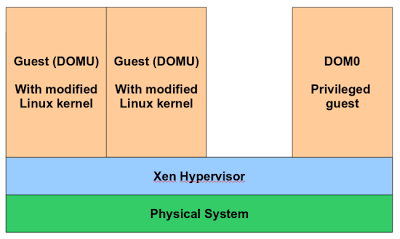
\includegraphics[width=8cm]{bilder/xen.png}
    \caption{Xen Architektur \citep{kvm:002}}
  \end{center}
\end{figure}

Als weitere Gastsysteme lassen sich wie auch bei KVM beliebige unmodifzierte Gastsysteme wie Linux-Distributionen oder Windows-Systeme installieren. Besonders ist aber, dass sich auch Linux-Distributionen mit ebenfalls modifiziertem Kernel laden lassen, die direkter mit dem Hypervisor zusammen arbeiten und so eine höhere Performance bieten.

\subsubsection{Hosted Hypervisors}

Ein Hosted Hypervisor ist ein \ac{VMM}, der als Anwendungsprogramm innerhalb eines Hostbetriebssystems läuft. Es ist somit möglich, auch andere Programme neben dem Hypervisor und seinen Gastbetriebssystemen zu verwenden.

\begin{figure}[!ht]
  \begin{center}
    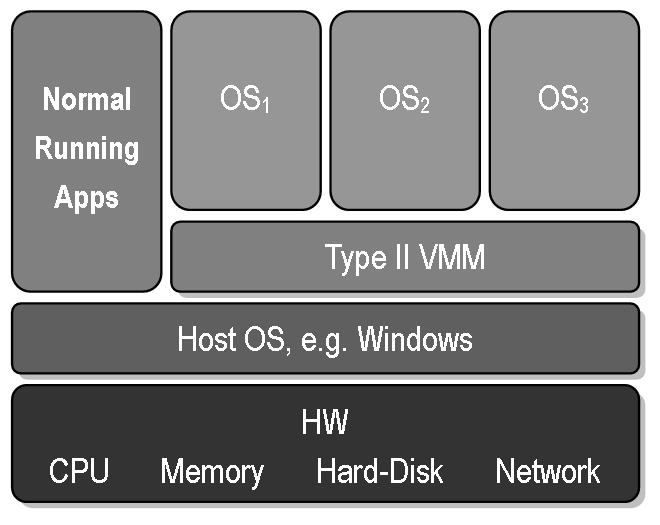
\includegraphics[width=6cm]{bilder/VMM-Type2.jpg}
    \caption{Virtual Machine Monitor Type II \citep{wiki:003}}
  \end{center}
\end{figure}

Größter Vorteil dieser Variante ist es also, dass das Hostsystem auch für gewöhnliche Benutzerarbeiten zur Verfügung steht und nicht ausschließlich zur Virtualisierung verwendet werden muss. Diese Virtualisierungslösung lässt sich sehr einfach nachträglich auf eine Vielzahl von Betriebssystemen installieren und auch wieder deinstallieren. Ein typische Vertreter dieser Hypervisor-Klasse ist zum Beispiel VirtualBox von Oracle \citep{wiki:004}.

\subsubsection{Unikernels}

Eine relativ neue Entwicklung innerhalb der Systemvirtualisierung mittels Hypervisor sind die sogenannten Unikernels. Vertreter dieser Idee kommen zum Beispiel aus dem Bereich der \ac{SOA} oder der Microservice Architecture. In diesen Architekturen wird versucht, die Teile eines IT-Systems als einzelne Dienste zu betrachten, die (meist über Netzwerk) miteinander kommunizieren. Es ist dabei von Vorteil, wenn diese Dienste jeweils eine bestimmte Aufgabe erledigen und über eine einfache Schnittstelle angesprochen werden können. Solche Dienste können nun jeweils über eine eigene \ac{VM} innerhalb der Virtualisierung abgebildet werden. Hierbei wird nun kritisiert, dass die Installation eines kompletten Gastbetriebssystems und die in ihm laufenden Anwendungsprogramme meist wesentlich mehr Resourcen und Programmcode verwenden und mehr Zugriffspunkte bieten, als für den eigentlichen Dienst benötigt wird. Als konzeptionelles Beispiel stellen wir uns hier einmal einen Dienst vor, der als einzige Aufgabe hat, mit Hilfe einer fortlaufenden Zahl neue Kundennummern zu generieren. Es ist nun durchaus nachvollziehbar, dass ein komplettes Gastbetriebssystem inkl. aller in ihm installierten Zubehörprogramme, Dokumentationen und Treiber sehr viel mehr Resourcen verbraucht, als für die eigentliche Operation sinnvoll erscheint. Die höhere Menge an Quellcode und typische Betriebssystemschnittstellen stellen zudem auch ein erhötes Sicherheitsrisiko dar, da sie potentiell mehr Angriffsvektoren bieten. Als Antwort entstehen deshalb in jüngster Vergangenheit neue Lösungen, bei denen man seinen eigentlichen Programmcode mit Hilfe einer Library entwickelt, die einfache Schnittstellen zur Verfügung stellt um z.B. Netzwerkkommunikation o.ä. zu betreiben. Der Programmcode wird dann mit Hilfe dieser Library in eine sehr viel kleinere \ac{VM} kompiliert, die wieder mit Hilfe eines Hypervisors ausgeführt werden kann. Ein Beispiel für eine solche Library ist MirageOS \citep[Vgl.][]{MadMorAnd13}.

\begin{figure}[!ht]
  \begin{center}
    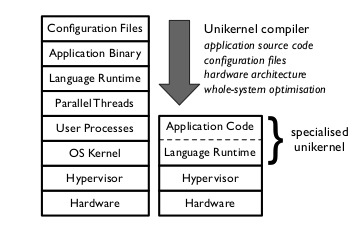
\includegraphics[width=8cm]{bilder/comparison-vm-unikernel.png}
    \caption{Vergleich klassische VM und Unikernel \citep[Abb. 1]{MadMorAnd13}}
  \end{center}
\end{figure}

Ein Nachteil dieser Lösung ist, dass man lediglich Funktionalität wiederverwenden kann, die genau durch die benutzte Library zur Verfügung steht. So kann man auch lediglich in der Programmiersprache arbeiten, die der Compiler der Library versteht. Im Falle von MirageOS ist dies die Sprache Ocaml. Es ist somit zum Beispiel nicht möglich, einen PHP-Interpreter zu starten und PHP-Scripte auszuführen, wie das mit allen gängigen Betriebssystemen wie Linux, MacOS oder Windows der Fall ist. Unikernels lassen sich somit zumindest bisher nur für sehr spezielle Dienste und Problemestellungen einsetzen.

\subsection{Betriebssystemvirtualisierung mittels OS-Containern}

Ein ganz anderer Ansatz als die Systemvirtualisierung mittels Hypervisor ist die sogenannte Betriebssystemvirtualisierung mittels OS-Container. Dabei wird nicht versucht, ein komplettes Gastsystem mit eigener, virtualisierter Hardware und eigenem Kernel auszuführen. Vielmehr wird grundsätzlich davon ausgegangen, dass sich alle virtuellen Betriebssysteme die Hardware und einen gemeinsamen Kernel teilen. Offensichtlich lassen sich damit nicht verschiedenste Betriebssysteme auf einer Maschine virtualisieren sondern immer nur Betriebssysteme, die auf dem gleichen Kernel basieren wie das Hostsystems. Dafür entfällt die Notwendigkeit, Hardware zu emulieren oder zu virtualisieren. In Bezug auf das Ring-Schemas des Prozessors gilt: Der gemeinsame Kernel arbeitet im Ring 0 und somit direkt auf der physischen Hardware. Das virtualisierte System beinhaltet lediglich Bibliotheken und Anwendungsprogramme und arbeitet somit in Ring 3. Die Notwendigkeit, nicht erlaubte Aufrufe zu finden und zu behandeln entfällt damit. Eine solche isolierte Umgebung, OS-Container genannt, gilt damit als grundsätzlich effizienter als komplette virtuelle Maschinen \citep[Vgl.][]{wiki:007}.

\begin{figure}[!ht]
  \begin{center}
    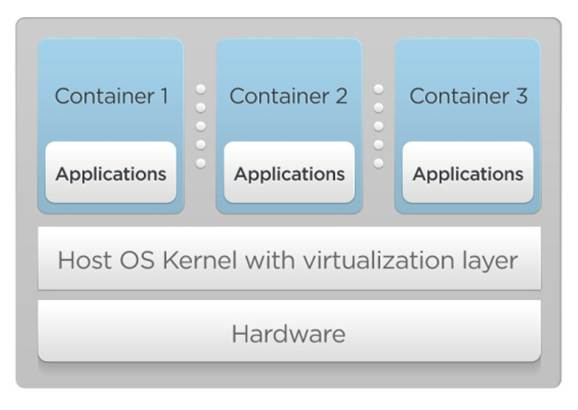
\includegraphics[width=8cm]{bilder/lxc-architecture.jpg}
    \caption{OS-Container \citep{Francis2014}}
  \end{center}
\end{figure}

Damit die einzelnen Container dennoch isoliert laufen und weder das Hostsystem noch andere Container manipulieren können, muss der Kernel spezielle Schnittstellen anbieten. Entsprechende Technologien sind im Laufe der Zeit bei einer Reihe von Betriebssystemen entwickelt worden, zum Beispiel auch für Linux und Windows. Für andere Betriebssysteme wiederum existiert keine entsprechende Schnittstelle, zum Beispiel Mac OS \citep[Vgl.][]{wiki:007}.

Ein prominenter Vertreter dieser Virtualisierungs-Art ist zur Zeit das Produkt Docker. Docker ist eine Open-Source-Plattform, mit deren Hilfe eine einfache Definition und Verwaltung solcher Container für den Linux-Kernel möglich ist. Kürzlich wurde aber auch eine Kooperation zwischen Microsoft und der Docker Inc., dem Unternehmen hinter Docker, bekannt gegeben. Ziel der Kooperation ist es unteranderem, dass sich entsprechende Container auch für Windows-Betriebssysteme erstellen lassen \citep[Vgl.][]{heise:001}.

Docker setzt auf eine Reihe von Schnittstellen auf, die inzwischen Teil des offizielen Linux-Kernels sind. Unter anderem gehören dazu die Cgroups und die Namespaces:

Cgroups (Control Groups) bieten die Möglichkeit, die Ressourcen-Nutzung bei der Ausführung von Prozessen durch den Kernel einzugrenzen. So lassen sich für Prozesse bestimmte Grenzen der Arbeitsspeicher- und Prozessor-Nutzung definieren. Außerdem lassen sich solche Prozesse auch komplett stoppen bzw. pausieren und wieder starten.

Kernel Namespaces erlauben es, die Sichtbarkeit von Prozessen untereinander einzugrenzen. So können über Namespaces zum Beispiel die Prozess-Identifikatoren (PIDs) für jeden Container neu vergeben werden. Jeder Container kann somit einen Prozess mit der ID 1 besitzen. Aber auch andere Aspekte des Betriebssystems, wie zum Beispiel Hostname, Benutzer-IDs, Dateisystem und Netzwerk-Zugriffe lassen sich mit den Kernel Namespaces von einander trennen.

Docker bietet zusätzlich ein weiteres nützliches Feature, sogenannte Union-Filesystems:

\begin{figure}[!ht]
  \begin{center}
    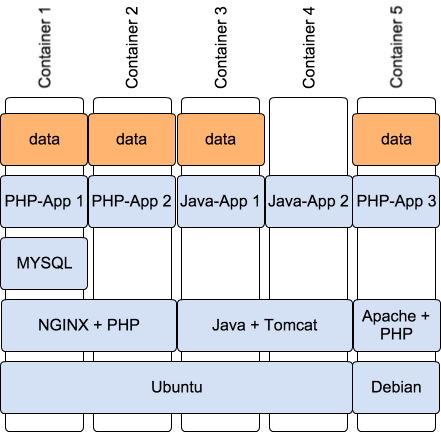
\includegraphics[width=8cm]{bilder/UnionFilesystem.png}
    \caption{Union Filesystem}
    \label{Union Filesystem}
  \end{center}
\end{figure}

Union-Filesystems sind Dateisysteme, die es erlauben, Dateisysteme transparent übereinander zu legen, um so weniger Speicherplatz zu verbrauchen. Das zugrundeliegende Verfahren nennt sich Copy-On-Write. Verwenden zwei Container zum Beispiel die gleiche Linux-Distrubution, so werden die entsprechenden Libraries und Anwendungsprogramme nur einmal auf der Festplatte vorgehalten. Das entsprechende Dateisystem wird dabei read-only unter ein für den Container beschreibbares Dateisystem gelegt. Die beiden Container unterscheiden sich also auf der Festplatte nur durch die tatsächlich individuell von ihnen geschriebenen Daten. Die meisten Union-Filesysteme erlauben dabei ein mehrfaches Übereinanderlegen, so dass eine ganze Hierarchie an ineinander verschachtelten Dateisystemen entstehen kann, um die Unterschiede zwischen den einzelnen Container maximal effizient auf der Festplatte abzulegen.

In der Abbildung \ref{Union Filesystem} wird zum Beispiel die gesamte Ubuntu-Distribution nur einmal auf der Festplatte abgelegt, obwohl sie von vier laufenden Containern verwendet wird. Sämtliche Dateisysteme sind read-only, bis auf die in rot angedeuteten Kästen, in denen die Container Laufzeitdaten speichern. Container 4 schreibt aber zum Beispiel keine Daten und ist somit komplett nur lesend.

\subsection{Vergleich}
